\documentclass[11pt,a4paper]{article}
\usepackage[margin=2.5cm]{geometry}
\usepackage{graphicx}
\usepackage{booktabs}
\usepackage{amsmath}
\usepackage{hyperref}
\usepackage{parskip}

\title{\textbf{Distributed Budgeted Maximum-Weight Clique}\\[4pt]
       \large MPI Branch-and-Bound: Parallelisation Strategy \& Scaling Results}
\author{Shahid Khan - 2022EE11163}
\date{}

\begin{document}
\maketitle

% ─────────────────────────────────────────────────────────────────────────────
\section*{Parallelisation Strategy}

The solver is an exact branch-and-bound (B\&B) with two pruning bounds:



\subsection*{Bitset-accelerated candidate sets}

Adjacency is stored as a flat contiguous array (\texttt{adj\_flat[N $\times$ WORDS]})
for cache-friendly row access.  The next candidate set after branching on $v$ is:
\[
  C_{\text{next}}[w] = C_{\text{rem}}[w] \;\mathbin{\&}\; \texttt{adj\_flat}[v \cdot \text{WORDS} + w]
\]
computed in $O(\lceil N/64 \rceil)$ word operations instead of an $O(k)$ linear scan.

Since $N\le1200$, bitsets never exceed 19 words (152 bytes). Candidate sets
use fixed-size \texttt{std::array} storage (19 \texttt{uint64\_t} words),
stack-allocated with zero heap allocation
in the hot recursive path.  Per-depth candidate arrays (\texttt{depth\_cand\_flat})
are pre-allocated once, eliminating \texttt{malloc}/\texttt{free} at every node.

\subsection*{Bucket sort for coloring bound}

Vertex profits satisfy $p(v)\in[1,100]$ (given by the problem constraints).
The coloring bound sorts candidates by profit before greedy class assignment.
Rather than \texttt{std::sort} ($O(k\log k)$), a counting/bucket sort over
the range $[1,100]$ runs in $O(k)$ and is used for this step.

\subsection*{Work distribution}

All vertices whose cost fits within $B$ form the \emph{initial candidate set}.
Each vertex in this set defines one independent first-level task (branch on that
vertex, search its subtree).

Tasks are distributed using \textbf{dynamic self-scheduling}:
a shared counter on rank~0 is decremented atomically via
\texttt{MPI\_Fetch\_and\_op} over a one-sided \texttt{MPI\_Win}.
Each rank repeatedly claims the next available task until the counter is
exhausted.  Because subtree sizes vary widely, this keeps all ranks busy
and avoids the idle time that static assignment produces when some subtrees
are much larger than others.  Below the first level, each rank runs its own
sequential B\&B with no further communication.

\subsection*{Asynchronous global lower-bound sharing}

Every rank maintains a local best profit $P_{\max}$.  The key insight is that
a higher $P_{\max}$ shared across all ranks means tighter pruning everywhere —
branches that cannot beat the global best are cut immediately.

\begin{itemize}
  \item \textbf{Sending:} whenever a rank finds a new best, it broadcasts
        the profit value to every other rank with a non-blocking
        \texttt{MPI\_Isend} — the search continues without waiting.
  \item \textbf{Receiving:} at the start of each B\&B node, the rank drains
        its message queue with \texttt{MPI\_Iprobe} + \texttt{MPI\_Recv},
        updating its local $P_{\max}$ if a better value arrived.
\end{itemize}

At the end, \texttt{MPI\_Allreduce} with \texttt{MPI\_MAXLOC} identifies
which rank holds the true global best clique.  That rank broadcasts the
vertex list and rank~0 writes the output file.

% ─────────────────────────────────────────────────────────────────────────────
\section*{Strong Scaling Results}

\begin{figure}[htbp]
  \centering
  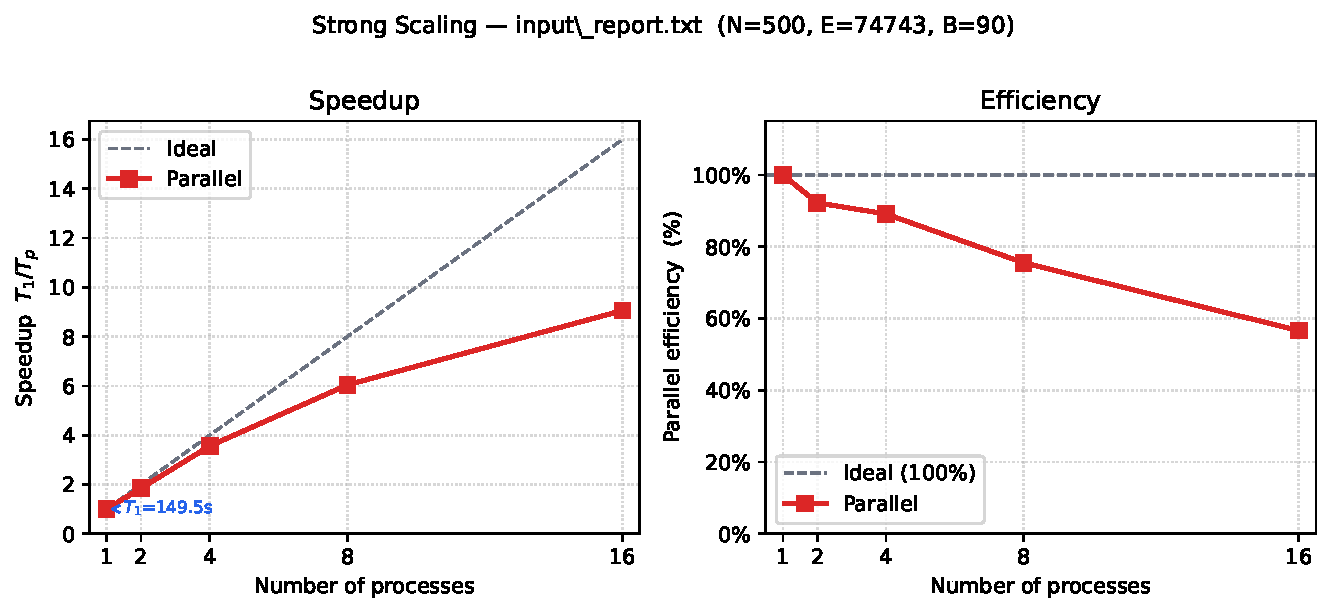
\includegraphics[width=\linewidth]{speedup_input_report.pdf}
  \caption{Strong scaling on \texttt{input\_report.txt} ($N=500$, $E=74{,}743$, $B=90$).
           Left: speedup $T_1/T_p$. Right: parallel efficiency.}
\end{figure}

\begin{table}[htbp]
\centering
\begin{tabular}{rrrr}
\toprule
Procs & $T$ (s) & Speedup & Efficiency \\
\midrule
1  & 8.130 & 1.000 & 100.0\% \\
2  & 4.770 & 1.704 &  85.2\% \\
4  & 2.760 & 2.946 &  73.6\% \\
8  & 1.640 & 4.957 &  62.0\% \\
16 & 1.250 & 6.504 &  40.7\% \\
\bottomrule
\end{tabular}
\caption{Timing on \texttt{input\_report.txt} ($N=500$, $E=74{,}743$, $B=90$).
         Efficiency drops at 16 ranks as communication overhead grows
         relative to the shrinking per-rank workload.}
\end{table}

\begin{figure}[htbp]
  \centering
  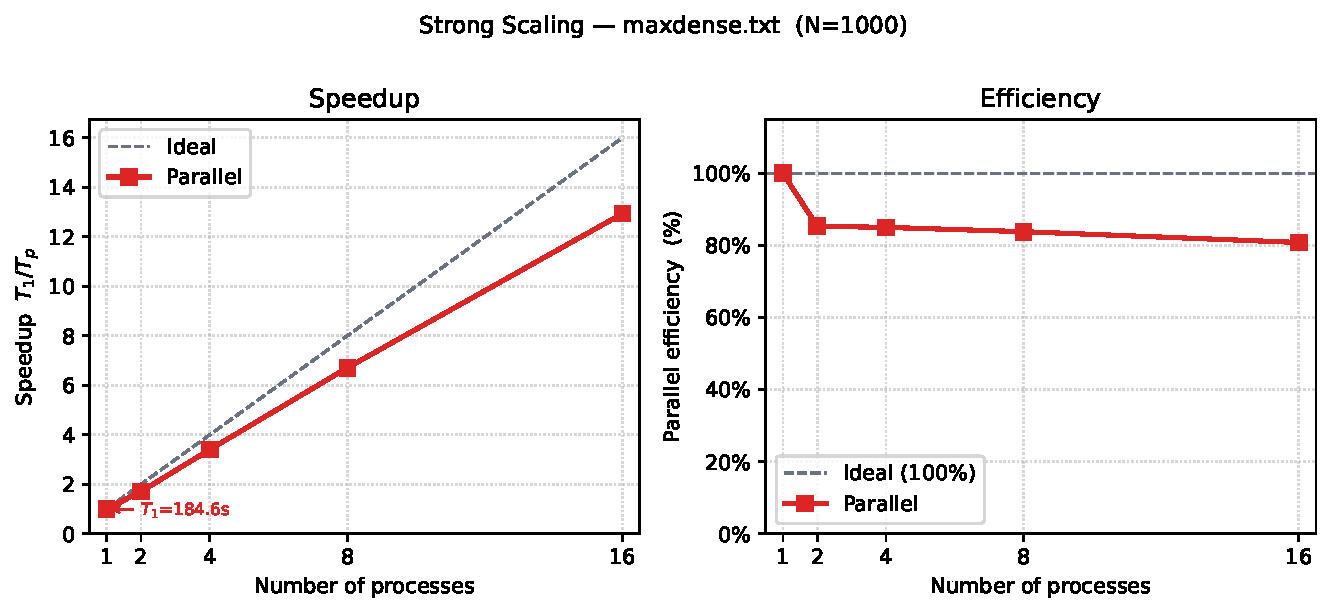
\includegraphics[width=\linewidth]{speedup_maxdense.pdf}
  \caption{Strong scaling on \texttt{maxdense.txt} ($N=1000$, $E = 249599$, $B=500$).
           Left: speedup $T_1/T_p$. Right: parallel efficiency.}
\end{figure}

\begin{table}[htbp]
\centering
\begin{tabular}{rrrr}
\toprule
Procs & $T$ (s) & Speedup & Efficiency \\
\midrule
1  & 184.630 & 1.000  & 100.0\% \\
2  & 108.237 & 1.706  &  85.3\% \\
4  &  54.280 & 3.401  &  85.0\% \\
8  &  27.531 & 6.706  &  83.8\% \\
16 &  14.275 & 12.934 &  80.8\% \\
\bottomrule
\end{tabular}
\caption{Timing on \texttt{maxdense.txt} ($N=1000$, $E = 249599$, $B=500$).
         Near-linear speedup up to 16 ranks due to the larger workload
         keeping all ranks busy throughout.}
\end{table}

This maxdense.txt can be downloaded from \href{https://drive.google.com/file/d/1v1EkGnd4ypIoKiQ6QbthsGpoGAFKPaxV/view?usp=sharing}{link}
% ─────────────────────────────────────────────────────────────────────────────
\end{document}
